%!TEX root = ../thesis.tex
\chapternumberfont{\fontsize{20pt}{20pt}\selectfont}
\chaptertitlefont{\fontsize{18pt}{18pt}\selectfont}

\chapter{Mainly introduce the methods and changes of citation, figures, headers and table}
\chaptermark{Introduction} % shown as header

\section{Mainly introduce the citation methods}

\textbf{Here is the first citation \cite{1_GCS2020}.}


"Sanhua Remi" (Japanese:sankare, Hong Kong and Taiwan translation: "How can zombies be so cute?" ) is a comic book serialized by Japanese cartoonist Hattori in Kodansha 's comic magazine " Bessatsu Shonen Magazine ". finished. There are derivative works such as animation. 

\textbf{Here is the two to four citations \cite{2_CA, 3_PSM, 4_HUANG2014}.}

The manga "Sanhua Reiya" is a manga series serialized by Japanese manga artist Hattori Hattori in Kodansha's manga magazine "Bessatsu Shonen Magazine". The work tells the story of the protagonist, Chihiro Fukutani, who accidentally made the dead heroine Sanhua Reya become a zombie due to the resurrection technique. In order to maintain Reya's body and realize her desire to become an "ordinary girl" "The story of the desire to run hard. It was serialized in the January 2010 issue of Kodansha's magazine "Bessatsu Shonen Magazine", and its special chapters were also published in irregular issues in "Weekly Shonen Magazine". It ended in the October issue of Weekly Shonen Magazine, which was released in September 2014.


\textbf{\textit{Here is the last citations \cite{5_Huang2020, 6_Huang2019}.}}

\section[The example of setting headers with longlonglonglong title]{The example of setting headers with longlonglonglong title%
  \sectionmark{The example set to short}}
\sectionmark{The example set to short}

Lorem ipsum dolor sit amet, consectetuer adipiscing elit. Ut purus elit, vestibulum ut, placerat ac, adipiscing vitae, felis. Curabitur dictum gravida mauris. Nam arcu libero, nonummy eget, consectetuer id, vulputate a, magna. Donec vehicula augue eu neque. Pellentesque habitant morbi tristique senectus et ne-
tus et malesuada fames ac turpis egestas. Mauris ut leo. 

% Table 1 from picture or you could manually create tables as shown in table 1.2
\begin{table}[htbp!]
  \caption[The name which will be shown on TOC]{The Figure names and figure legends. \textbf{(a)} ahahda dqwe ead asd. \textbf{(b-d)} ahahda dqwe ead asd.}
  \centering
  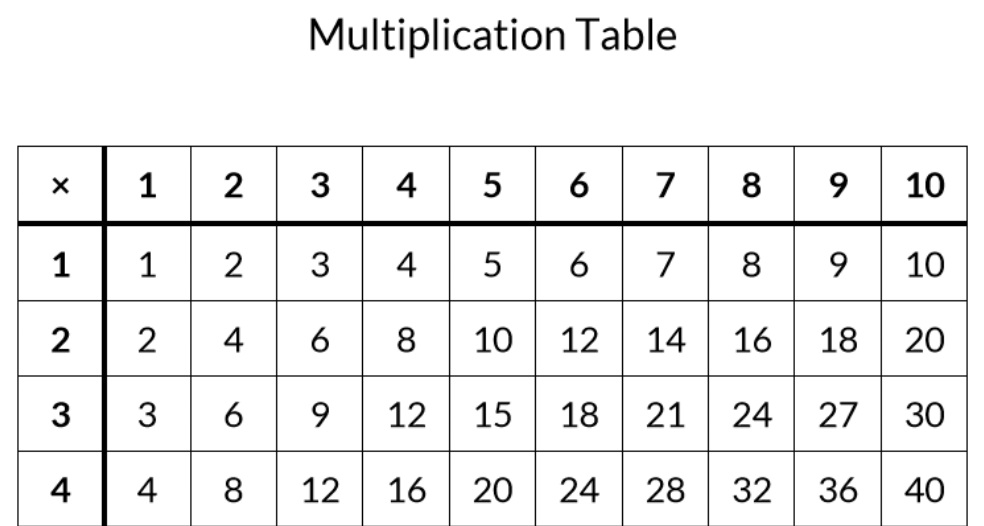
\includegraphics[width=1\textwidth]{Table 1.1} % the table figure name 
  % \label{tab1.1} not used here
\end{table}

\lipsum[1]

% Table 1.2
\begin{table}
\caption{Even better looking table using booktabs}
\centering
\label{table:good_table}
\begin{tabular}{l c c c c}
\toprule
\multirow{2}{*}{Dental measurement} & \multicolumn{2}{c}{Species I} & \multicolumn{2}{c}{Species II} \\
\cmidrule{2-5}
  & mean & SD  & mean & SD  \\
\midrule
I1MD & 6.23 & 0.91 & 5.2  & 0.7  \\

I1LL & 7.48 & 0.56 & 8.7  & 0.71 \\

I2MD & 3.99 & 0.63 & 4.22 & 0.54 \\

I2LL & 6.81 & 0.02 & 6.66 & 0.01 \\

CMD & 13.47 & 0.09 & 10.55 & 0.05 \\

CBL & 11.88 & 0.05 & 13.11 & 0.04\\
\bottomrule
\end{tabular}
\end{table}

% figure 1.1, the afterpage methods always put the figure at the top of new page.
\afterpage{
    \centering
    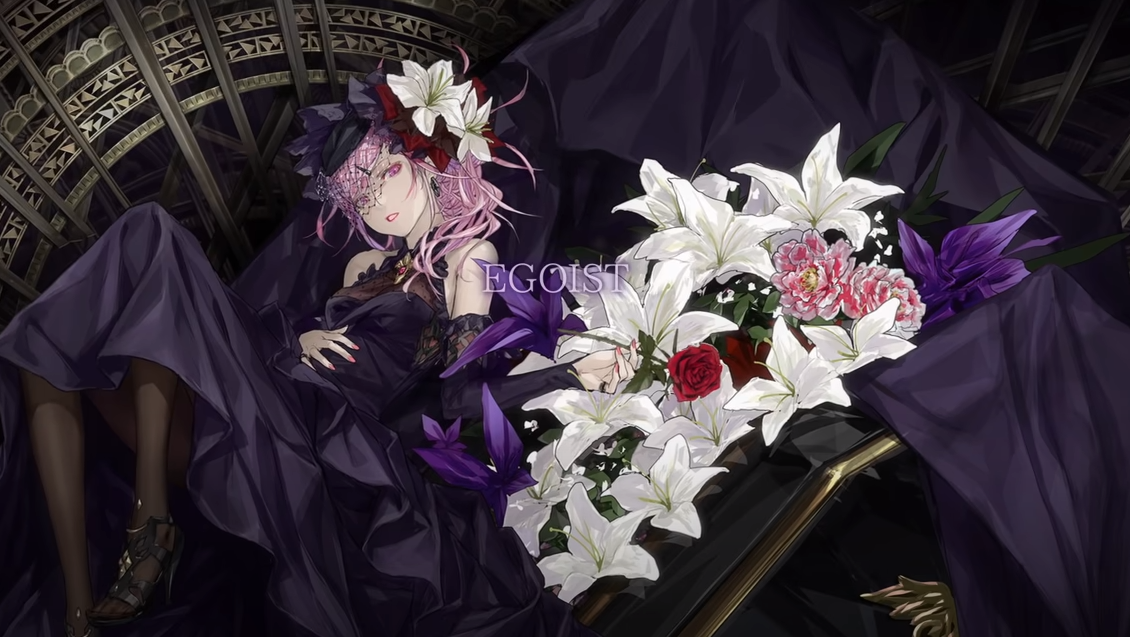
\includegraphics[width=1\textwidth]{Figure 1.1}
    \captionsetup{parbox=none}
    \captionof{figure}[Examples of something here to shown the afterpage figure methods.]{\textbf{Examples of something here to shown the afterpage figure methods.} \textbf{(a)} A hematoxylin and eosin (H{\&}E)-stained whole-slide image \textbf{(b)} Examples of something here to shown the afterpage figure methods. \textbf{(c)} Examples of something here to shown the afterpage figure methods.}
    % \vspace{\intextsep}
}

Lorem ipsum dolor sit amet, consectetuer adipiscing elit. Ut purus elit, vestibulum ut, placerat ac, adipiscing vitae, felis. Curabitur dictum gravida mauris. Nam arcu libero, nonummy eget, consectetuer id, vulputate a, magna. Donec vehicula augue eu neque. Pellentesque habitant morbi tristique senectus et ne-
tus et malesuada fames ac turpis egestas. Mauris ut leo. Lorem ipsum dolor sit amet, consectetuer adipiscing elit. Ut purus elit, vestibulum ut, placerat ac, adipiscing vitae, felis. Curabitur dictum gravida mauris. Nam arcu libero, nonummy eget, consectetuer id, vulputate a, magna. Donec vehicula augue eu neque. Pellentesque habitant morbi tristique senectus et netus et malesuada fames ac turpis egestas. Mauris ut leo. Lorem ipsum dolor sit amet, consectetuer adipiscing elit. Ut purus elit, vestibulum ut, placerat ac, adipiscing vitae, felis. Curabitur dictum gravida mauris. Nam arcu libero, nonummy eget, consectetuer id, vulputate a, magna. Donec vehicula augue eu neque. Pellentesque habitant morbi tristique senectus et netus et malesuada fames ac turpis egestas. Mauris ut leo. Lorem ipsum dolor sit amet, consectetuer adipiscing elit. Ut purus elit, vestibulum ut, placerat ac, adipiscing vitae, felis. Curabitur dictum gravida mauris. Nam arcu libero, nonummy eget, consectetuer id, vulputate a, magna. Donec vehicula augue eu neque. Pellentesque habitant morbi tristique senectus et netus et malesuada fames ac turpis egestas. Mauris ut leo.

% Figure 1.2  the begin{figure} method could put into any place if the space is enough on the current page.
\begin{figure}[htbp!]
  \centering
  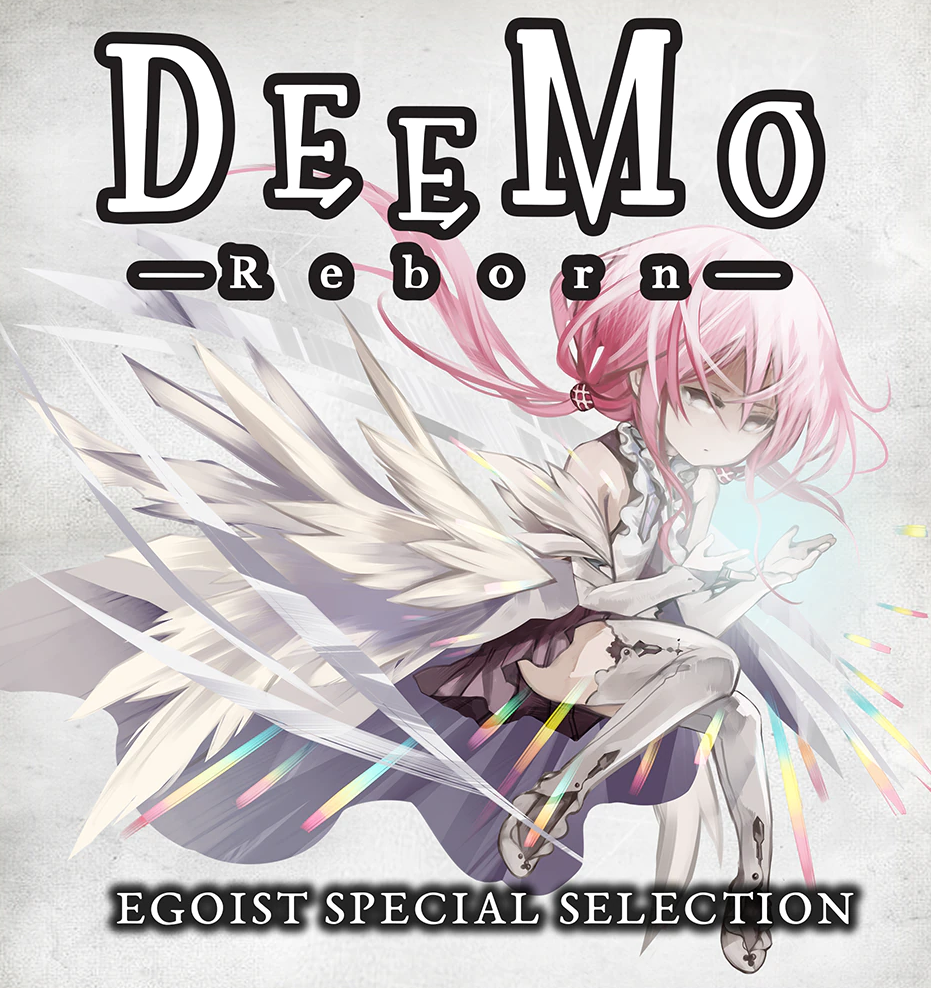
\includegraphics[width=0.7\textwidth]{Figure 1.2}
  \caption[the begin{figure} method could put into any place if the space is enough on the current page.]{\textbf{the begin{figure} method could put into any place if the space is enough on the current page. But figure 1.2 did not have the enough space to put on the current pages.} the begin{figure} method could put into any place if the space is enough on the current page. But figure 1.2 did not have the enough space to put on the current pages. the begin{figure} method could put into any place if the space is enough on the current page.the begin{figure} method could put into any place if the space is enough on the current page.the begin{figure} method could put into any place if the space is enough on the current page.}
  \end{figure}


\section{Objectives of the Study}

The overall goal of this study is to dissect and further investigate the association with  based on . 

An efficient and robust Comic framework is proposed to dissect the purity of users. The detailed description and results of our exploration will be introduced in \textbf{Chapter 2}.


Next, a deep learning framework-Game Center is designed for fully automated user classification through transfer learning from Anime. Our exploration will be detailed in \textbf{Chapter 3}.


The multi-omics Novel subtyping is translated into the clinic by developing a light novel classification system. These interesting studies will be discussed in \textbf{Chapter 4}.


% Figure 1.2  the begin{figure} method could put into any place if the space is enough on the current page.
\begin{figure}[htbp!]
  \centering
  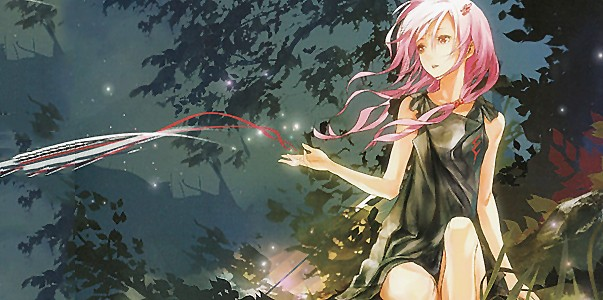
\includegraphics[width=1\textwidth]{Figure 1.3}
  \caption[But figure 1.2 did not have the enough space to put on the current pages]{\textbf{the begin{figure} method could put into any place if the space is enough on the current page.}}
  \end{figure}



\section{Thesis outline}

\begin{itemize}
    \item \textbf{Chapter1:} Introduction to .
    \item \textbf{Chapter2:} Identification of in Microenvironment using Deep Learning.
    \item \textbf{Chapter3:} Deep Learning-derived analysis on .
    \item \textbf{Chapter4:} Multi-Omics Novel subtyping of light novel using Deep Learning.
    \item \textbf{Chapter5:} Conclusion and Future Prospective.
\end{itemize}